\documentclass[12pt,a4paper,titlepage]{scrartcl}

\usepackage{comment}
\usepackage[main=ngerman,english]{babel}
\usepackage[utf8]{inputenc}
\usepackage[T1]{fontenc}
\usepackage{lmodern}
\usepackage{geometry}
\geometry{left=2.5cm,right=2.5cm,top=2.5cm,bottom=3cm,head=29pt,foot=25pt}
\setlength{\footheight}{25pt}
\usepackage{microtype}
\usepackage{amsmath,amssymb,mathtools}
\numberwithin{equation}{section}
\numberwithin{table}{section}
\numberwithin{figure}{section}
\usepackage{siunitx}
\sisetup{locale=DE, separate-uncertainty=true, per-mode=fraction}
\usepackage{booktabs}
\usepackage{multirow}
\usepackage{graphicx}
\usepackage{float}
\usepackage{caption}
\usepackage{subcaption}
\usepackage[automark]{scrlayer-scrpage}
\usepackage[most]{tcolorbox}
\usepackage{hyperref}
\usepackage{pdfpages}
\usepackage{csvsimple-l3}
\usepackage{longtable}
\usepackage{graphicx}


\hypersetup{colorlinks=true, linkcolor=blue!60!black, urlcolor=blue!60!black, citecolor=blue!60!black}

\clearpairofpagestyles

\chead{%
    \versuch\hfill\autor\\
    \rule{\textwidth}{0.2pt}%
}
\cfoot{%
    \rule{\textwidth}{0.2pt}\\[-0.5ex]
    \pagemark\ 
}
\addtokomafont{pagefoot}{\small}
\setlength{\parindent}{0pt}


\newtcolorbox{resultbox}[1][]{ 
    enhanced,
    colback=black!4!white,
    colframe=black!65!black,
    boxrule=0.8pt,
    arc=0.0mm,
    title=#1,
    fonttitle=\bfseries,
    %drop shadow
}


\newcommand{\versuch}{Versuch 23}
\newcommand{\titel}{Strom- und Spannungsmessung}
\newcommand{\praktikum}{Physikalisches Anfängerpraktikum 1}
\newcommand{\autor}{Jonathan Gießen}
\newcommand{\gruppe}{Gruppe 8}
\newcommand{\datum}{2. September 2026}
\newcommand{\betreuer}{Julius Laub}

\begin{document}

\pagestyle{scrheadings}

\begin{titlepage}



    \centering
    \vspace*{4cm}
    {\large Universität Heidelberg\par}
    {\small Fakultät für Physik und Astronomie\par}
    {\Large \praktikum\par}
    \vspace{0.8cm}
    {\LARGE \bfseries \versuch\ -- \titel\par}
    \vspace{1.5cm}

    \begin{tabular}{ll}
        \textbf{Autor:} & \autor\\
        \textbf{Gruppe:} & \gruppe\\
        \textbf{Betreuer:} & \betreuer\\
        \textbf{Versuchsdatum:} & \datum\\
    \end{tabular}

    \vfill
    \hrulefill\
\end{titlepage}

\tableofcontents

\clearpage
\section{Einleitung}
Der Versuch 23 \glqq\ Strom- und Spannungsmessung\grqq\ beschäftigt sich
mit der Untersuchung von Strom- und Spannungsmessungen in Gleichstromkreisen.
Ein zentrales physikalisches Problem der elektrischen Messtechnik ist, dass reale Messgeräte und Spannungsquellen
von Idealwerten abweichen.  Jedes reale Messgerät, wie das in diesem Versuch verwendete Drehspulinstrument,
besitzt einen eigenen Innenwiderstand, der unweigerlich die zu messende Schaltung beeinflusst und das Messergebnis verfälscht.
Ein erstes Zeil dieses Versuchs ist es daher, diesen systematischen Fehler anhand eines Spannungsteilers praktisch zu erkennen.
\medspace\ 

Zudem wird gezeigt, wie der Messbereich von Volt- und Amperemetern durch die gezielte Beschaltung mit Parallel- und Serienwiderständen
theoretisch berechnet und experimentell erweitert werden kann.  Um den verfälschenden Einfluss des Messgeräte-Innenwiderstands bei der 
Spannungsmessung vollständig zu umgehen, wird im weiteren Verlauf eine Kompensationsschaltung aufgebaut und mithilfe einer Präzisionsspannungsquelle geeicht. 
Diese Schaltung ermöglicht durch eine Gegenspannung eine nahezu stromlose – und damit exakte – Bestimmung von elektrischen Spannungen.  
Abschließend wird diese präzise Messmethode angewandt, um das Verhalten einer Batterie (reale Spannungsquelle) unter Belastung zu charakterisieren.
Durch die Messung der Klemmenspannung bei verschiedenen, gezielt eingestellten Entnahmeströmen von bis zu 200 mA lassen sich die Quellenspannung und der Innenwiderstand der Batterie experimentell bestimmen

\section{Grundlagen und Theorie}


\subsection{Literaturwerte}





\section{Messprotokoll}

\subsection{Versuchsaufbau und Aufgaben}
\begin{comment}
    
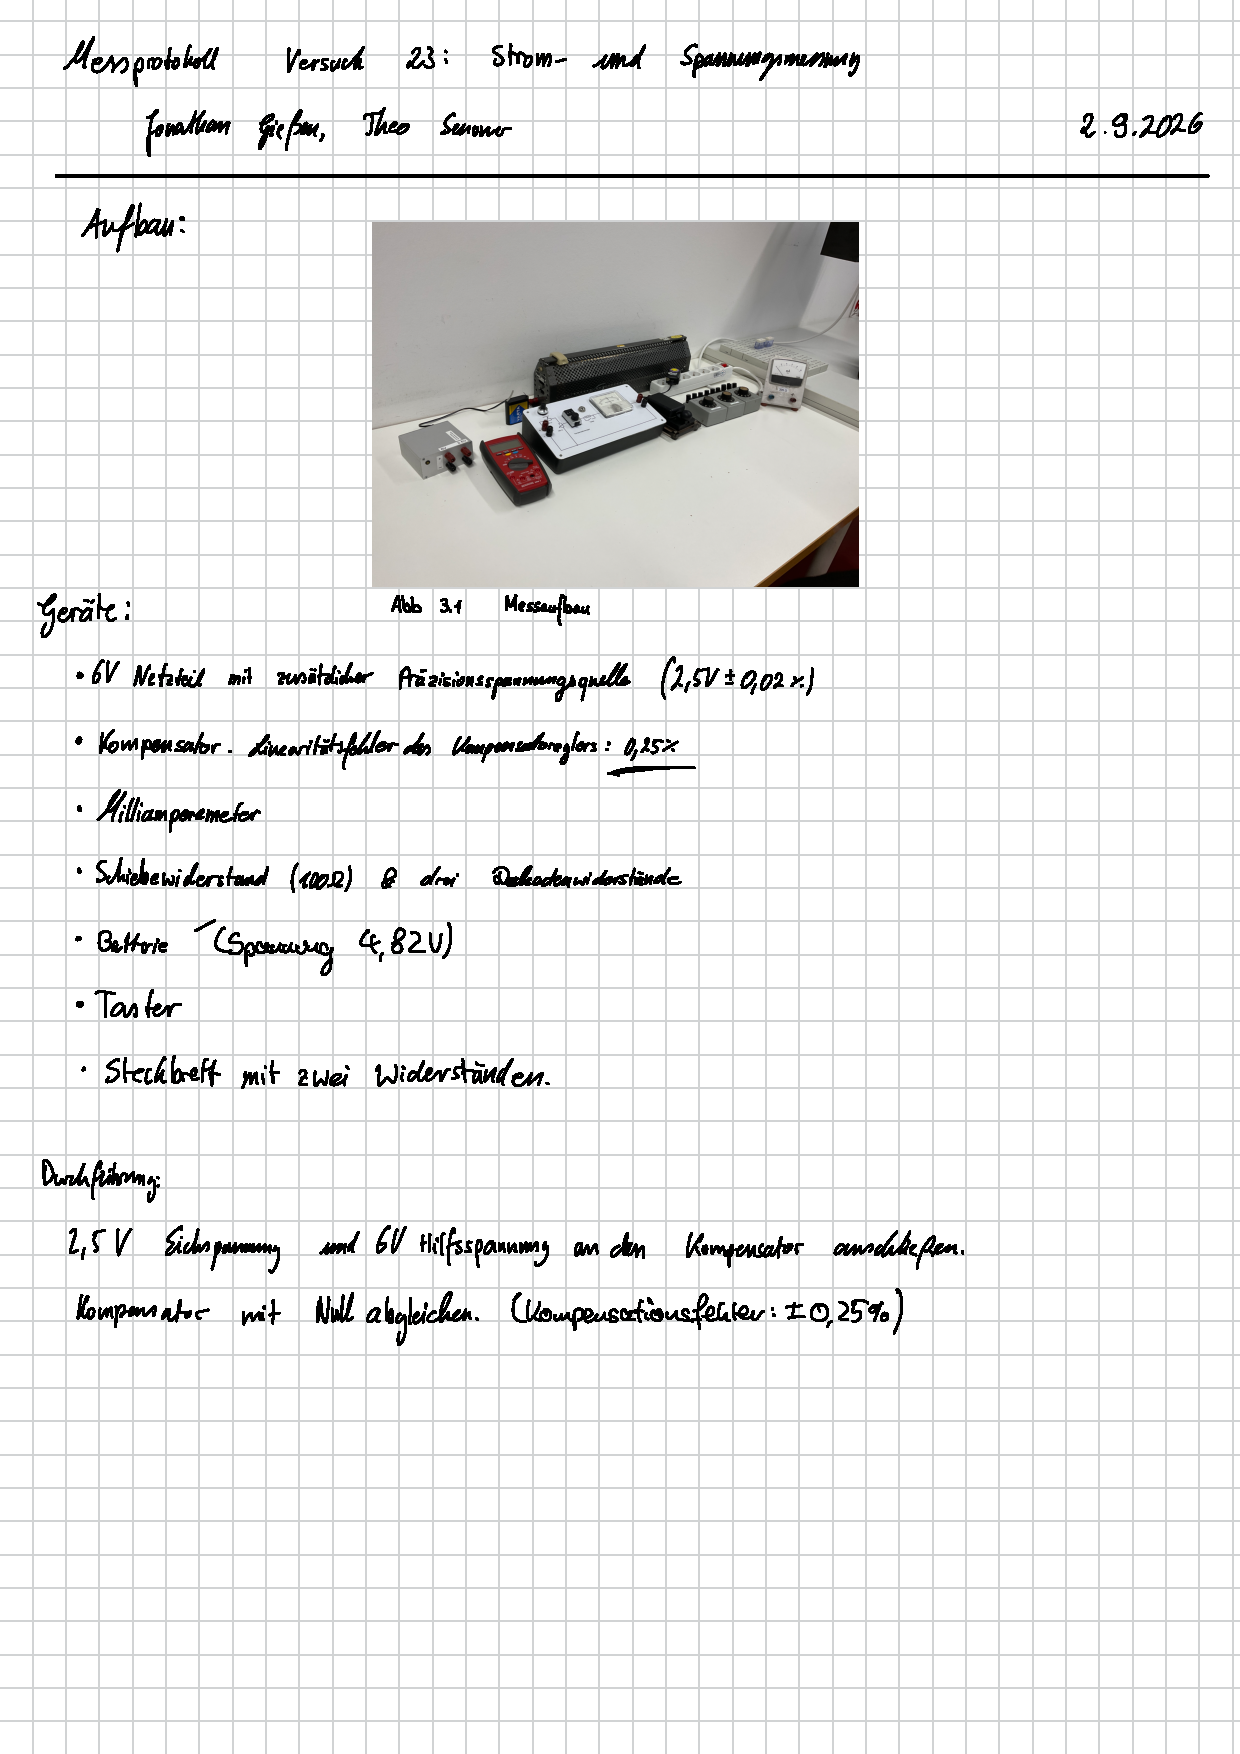
\includepdf[
    pages=-,
    width=\textwidth,
    height=\textheight,
    keepaspectratio,
    pagecommand={\thispagestyle{scrheadings}}
]{../Messprotokoll 23.pdf}

\end{comment}

\addtocounter{figure}{1}

\subsection{Durchführung}

\subsection{Messwerte}




\section{Auswertung}

\subsection{Aufgabe 1:Exemplarische Berechnung an einem ausgewählten Tröpfchen}

\begin{comment}
\begin{table}[H]
    \centering
    \caption{Mess- und Geräteparameter für die exemplarische Berechnung (Messung 28).}
    \label{tab:parameter_messung_28}
    \begin{tabular}{ll}
        \toprule
        \textbf{Größe} & \textbf{Wert} \\
        \midrule
        Fallstrecke & $s_1 = 10\,\text{Skt} = 5.00 \cdot 10^{-4}\,\text{m}$ \\
        Fallzeit & $t_1 = 11.85\,\text{s}$ \\
        Steigstrecke & $s_2 = 10\,\text{Skt} = 5.00 \cdot 10^{-4}\,\text{m}$ \\
        Steigzeit & $t_2 = 18.19\,\text{s}$ \\
        Skalenteilung & $1\,\text{Skt} = 5.00 \cdot 10^{-5}\,\text{m}$ \\
        Kondensatorspannung & $U = 500\,\text{V}$ \\
        Plattenabstand & $d = 6.00 \cdot 10^{-3}\,\text{m}$ \\
        Luftdruck & $p = 100285\,\text{Pa}$ \\
        Erdbeschleunigung & $g = 9.81\,\frac{\text{m}}{\text{s}^2}$ \\
        Dichtedifferenz & $\rho = \rho_{\text{Öl}} - \rho_{\text{Luft}} = 871.21\,\frac{\text{kg}}{\text{m}^3}$ \\
        Unkorrigierte Luftviskosität & $\eta_0 = 1.81 \cdot 10^{-5}\,\text{Pa}\cdot\text{s}$ \\
        Cunningham-Konstante & $b = 7.78 \cdot 10^{-3}\,\text{Pa}\cdot\text{m}$ \\
        \bottomrule
    \end{tabular}
\end{table}
\end{comment}

\begin{comment}
    
\medskip
\begin{resultbox}[Ergebnis der exemplarischen Berechnung]
    Die exemplarisch berechneten Werte für Messung Nr.~28 lauten:
    \begin{align*}
        v_f &= 4.219 \cdot 10^{-5}\,\frac{\text{m}}{\text{s}}, \\
        v_s &= 2.749 \cdot 10^{-5}\,\frac{\text{m}}{\text{s}}, \\
        r_0 &= 6.341 \cdot 10^{-7}\,\text{m}, \\
        f(r_0) &= 0.891, \\
        q &= 1.521 \cdot 10^{-19}\,\text{C}.
    \end{align*}
    Ein Vergleich mit Zeile 28 der generierten Auswertungstabelle zeigt, dass sämtliche handgerechneten Werte exakt mit den Ausgabewerten von Excel übereinstimmen.

\end{resultbox}
    
\end{comment}


\subsection{Aufgabe 2: Histogramm der gemessenen Ladungen}



\subsection{Systematische Fehlerabschätzung der Tröpfchenladung}

Zur Abschätzung der relativen systematischen Messunsicherheit $\frac{\Delta q}{q}$ wird die Gauß'sche Fehlerfortpflanzung auf die Bestimmungsgleichung der Ladung angewendet:
\begin{equation}
    q = (v_f + v_s) \cdot \frac{6\pi d}{U} \sqrt{\frac{9 v_f \eta^3}{2\rho g}}
    \label{eq:q_exakt}
\end{equation}

\begin{comment}
\begin{table}[H]
    \centering
    \caption{Relative Unsicherheiten der Eingangsgrößen.}
    \begin{tabular}{lll}
        \toprule
        \textbf{Größe} & \textbf{Relative Unsicherheit} & \textbf{Wert} \\
        \midrule
        Strecke $s$ & $\dfrac{\Delta s}{s}$ & $\dfrac{0.13 \cdot 10^{-5}\,\text{m}}{5.00 \cdot 10^{-5}\,\text{m}} = 2.60\,\% = 0.0260$ \\
        Viskosität $\eta$ & $\dfrac{\Delta \eta}{\eta}$ & $2.0\,\% = 0.020$ \\
        Dichte $\rho$ & $\dfrac{\Delta \rho}{\rho}$ & $0.5\,\% = 0.005$ \\
        Plattenabstand $d$ & $\dfrac{\Delta d}{d}$ & $\dfrac{0.05\,\text{mm}}{6.00\,\text{mm}} \approx 0.833\,\% = 0.00833$ \\
        Spannung $U$ & $\dfrac{\Delta U}{U}$ & $0.5\,\% = 0.005$\footnotemark \\
        \bottomrule
    \end{tabular}
\end{table}
\footnotetext{Für die systematische Unsicherheit der Spannungsmessung wird gemäß Aufgabenstellung eine relative Unsicherheit von $0.5\,\%$ angenommen,
was bei $U = 500\,\text{V}$ einer systematischen Geräteunsicherheit von $\Delta U_{\text{sys}} = \pm 2.5\,\text{V}$ entspricht.
Die im Messprotokoll notierte Unsicherheit von $\pm 4\,\text{V}$ berücksichtigt darüber hinaus die beobachtete statistische Schwankung sowie die thermische Drift der Hochspannungsquelle über den gesamten Messzeitraum.}
\end{comment}

\subsection{Abschätzung des statistischen Fehlers aus der Mehrfachmessung}


\subsection{Vergleich des Ergebnisses mit dem Literaturwert}



\section{Diskussion}
\subsection{Interpretation der Signifikanzen}

\medskip
\noindent

\subsection{Fazit}
Zum Ende lässt sich festhalten, dass die experimentelle Bestimmung der Elementarladung mit dem Millikan-Versuch 
erfolgreich durchgeführt wurde. Die Ergebnisse stimmen innerhalb der Unsicherheiten mit dem Literaturwert überein, und die Analyse der Fehlerquellen liefert wertvolle 
Einblicke in die Genauigkeit und Präzision des Versuchsaufbaus.

\clearpage

\listoffigures


\listoftables

\begin{thebibliography}{5}
    \bibitem{PAPskript} Dr. J.Wagner, \emph{Physikalisches Anfängerpraktikum}, Stand 11/2024
    \bibitem{ilberg1988physikalisches} W. Ilberg, M. Krötzsch, \emph{Physikalisches Praktikum für Anfänger}, BSB B. G. Teubner Verlagsgesellschaft, Leipzig (1985).
    \bibitem{demtroeder2017} W. Demtröder, \emph{Experimentalphysik 1: Mechanik und Wärme}, Springer Verlag, Berlin (2017).
\end{thebibliography}



\begin{tcolorbox}[colback=gray!5,colframe=gray!60,boxrule=0.8pt,arc=0.01mm,title=KI-Hinweis]
    Für die sprachliche Formulierung dieses Protokolls wurde in Teilen KI-gestützte Textgenerierung verwendet. 
\end{tcolorbox}

\end{document}